\documentclass[11pt]{beamer}
\usepackage{amsfonts,amsmath,amsthm,amssymb}
\theoremstyle{plain}
\newtheorem{conjecture}{Conjecture}[section]
\usepackage{mathtools,mathptmx,listings,forest,enumitem}
\usepackage{graphicx}
\usepackage{pgfplots}
\pgfplotsset{compat=newest}
% plotting things
\usepackage{graphicx}
\graphicspath{{images/}}
\usepackage{tikz-cd}
\pgfplotsset{compat=1.15}
\usepackage[
	backend=biber,
	style=verbose,
	sorting=ynt
]{biblatex}
\addbibresource{references.bib}
\usetheme{Madrid}
\usepackage{float,mathtools,dirtytalk,ulem,csquotes,cancel,hyperref}
\author[] % (optional)
{Emon Hossain\inst{1}}

\institute[University of Dhaka] % (optional)
{
  \inst{1}%
  Lecturer\\MNS department\\Brac University
}

\date[] % (optional)
{\textsc{Lecture-03}}


\title[]{MAT215: Complex Variables And Laplace Transformations}

\setbeamertemplate{navigation symbols}{}


\AtBeginSection[]
{
  \begin{frame}
    \frametitle{Table of Contents}
    \tableofcontents[currentsection]
  \end{frame}
}

\usepackage{Kyushu}

% \usetheme{Frankfurt}

\begin{document}
% \begin{frame}
% \titlepage
% \end{frame}

% \begin{frame}{Example}
%     \begin{example}
%         Evaluate $$\int_C (x^2-iy^2)dz$$
%         \begin{itemize}
%             \item (a) Along the parabola $y=2x^2$ from $(1,2)$ to $(2,8)$
%             \item (b) Along the straight line from $(1,2)$ to $(2,8)$
%             \item (c) Along the straight lines from $(1,2)$ to $(1,8)$ and then from $(1,8)$ to $(2,8)$
%         \end{itemize}
%     \end{example}
%     \textbf{Hint:} Let's identify how many steps we need to do this kind of math:
%     \begin{itemize}
%         \item Find parametrization
%         \item Find the limit for the parameter
%         \item Rewrite the expression in terms of the parameter
%     \end{itemize}
% \end{frame}

% \begin{frame}{continue}
%     Use the formula to have the parametric representation of the curve $C$, 
%     $$\boxed{\text{Explicit function: }\gamma(t)\stackrel{y=f(x)}{=}(t,f(t))}$$
%     and
%     $$\boxed{\text{Line segment: }\gamma(t)= a+t(b-a), 0\leq t\leq 1}$$
%     Now, use 
%     $$
%     \int_C f(z) dz=\int_a^b f(\gamma(t))\gamma'(t)dt
%     $$
%     Do the answers of $(b)$ and $(c)$ give you any insight into the analyticity? 
% \end{frame}

% \begin{frame}{Example}
%     Evaluate $$\oint_C |z|^2 dz$$
%     around the square with vertices at $(0,0), (1,0), (1,1)$ and $(0,1)$.\\
%     \textbf{Hint:} You could parametrize each side and sum, but Green’s theorem makes it a one-liner.
%     $$\oint_C Pdx+Qdy\stackrel{?}{=}\iint_A \left( \frac{\partial Q}{\partial x}-\frac{\partial P}{\partial y} \right) dxdy$$
%     If you understand why the line integral and the area integral are equal, have a look at \url{https://www.youtube.com/watch?v=8SwKD5_VL5o}.
% \end{frame}

% \begin{frame}{Example}
%     Evaluate $$\oint (\bar z)^2 d z$$
%     around the circles $(a)$ $|z|=1$ and $|z-1|=1$.\\
%     \textbf{Hint:} For $|z-z_0|=r$ instead of using $\gamma(t)=(\cos t,\sin t)$, use $z-z_0=r e^{i\theta}$.   
% \end{frame}

% \begin{frame}{Example}
%     Verify that, $$\oint_C z^2 dz=0$$
%     Where $C$ is the boundary of the triangle with vertices $(0,0)$, $(1,1)$ and $(0,1)$. 
% \end{frame}

\begin{frame}{Cauchy-Goursat Theorem}
    \textbf{Statement:} Let $f(z)$ be analytic in a region $R$ and on its boundary $C$. Then $$\oint_C f(z) dz=0$$
\end{frame}

\begin{frame}{Example}
    Evaluate $$\oint_C \frac{z^2}{z-1}dz$$
    where $C$ is the circle $|z-2|=3$.\\
    \textbf{Hint:} Use path deformation, $$|z-2|=3\rightarrow |z-1|=1$$ 
\end{frame}

\begin{frame}{Example}
\textbf{Interesting question:}
    Evaluate
$$
\oint_C \frac{1}{z-a} d z
$$
Where $C$ is any simple closed curve and\\
i) $z=a$ is outside $C$\\
ii) $z=a$ is inside $C$
\end{frame}

\begin{frame}{Example}
\textbf{Interesting question:}
    Evaluate
$$
\oint_C \frac{1}{(z-a)^{n+1}} d z
$$
Where $C$ is any simple closed curve and\\
i) $z=a$ is outside $C$\\
$$\oint_C \frac{1}{(z-a)^{n+1}} d z=0$$
ii) $z=a$ is inside $C$
$$
\oint_C \frac{1}{(z-a)^{n+1}} d z=\begin{cases}
    2\pi i,&n=0\\
    0,&n> \text{otherwise}
\end{cases}
$$
\end{frame}

% \begin{frame}{Cauchy Integral Formula}

% \begin{figure}
%     \centering
%     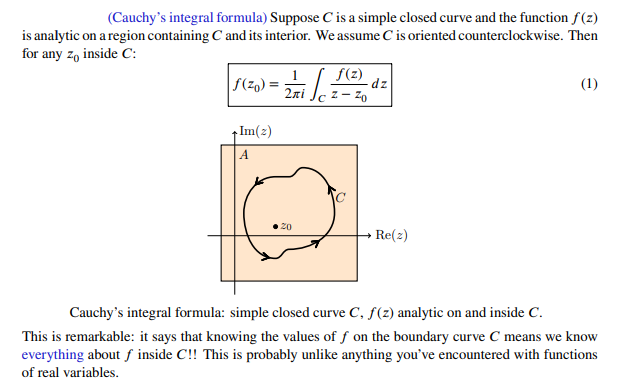
\includegraphics[width=\linewidth]{Screenshot 2025-09-04 104432.png}
% \end{figure}
% \end{frame}

% \begin{frame}{Example}
%     \begin{figure}
%         \centering
%         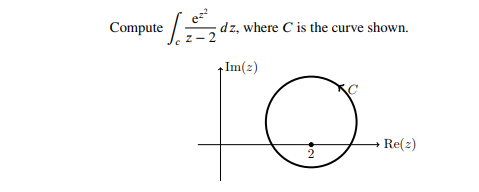
\includegraphics[width=1\linewidth]{Screenshot 2025-09-04 104237.png}
%     \end{figure}
% \end{frame}

% \begin{frame}{Example}
%     \begin{figure}
%         \centering
%         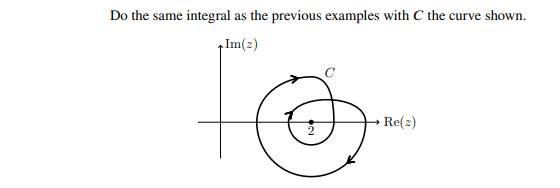
\includegraphics[width=1\linewidth]{Screenshot 2025-09-04 104251.png}
%     \end{figure}
% \end{frame}

\begin{frame}{Example}
    \begin{figure}
        \centering
        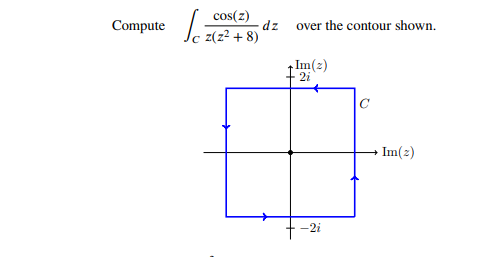
\includegraphics[width=1\linewidth]{Screenshot 2025-09-04 104207.png}
    \end{figure}
\end{frame}

\begin{frame}{Example}
    \begin{figure}
        \centering
        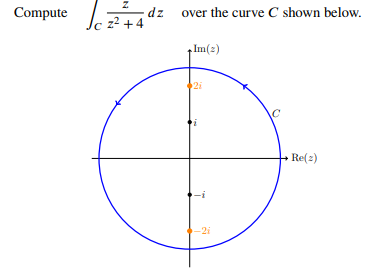
\includegraphics[width=1\linewidth]{Screenshot 2025-09-04 104827.png}
    \end{figure}
\end{frame}

\begin{frame}{General version}
    \textbf{General version:}
$$
f^n(a)=\frac{n!}{2 \pi i} \oint_C \frac{f(z)}{(z-a)^{n+1}} d z
$$
\textbf{Example:} 
$$
\text { Evaluate } \oint_C \frac{e^z}{\left(z^2+\pi^2\right)^2} d z \text { where } C \text { is the circle }|z-i|=4
$$
$$\boxed{\text{Did you notice that for multiple poles we can use partial fractions?}}$$
We have a better method to handle that!
\end{frame}

\begin{frame}{Behavior of functions near zeros and poles}
    The basic idea is that near a zero of order $n$, a function behaves like $(z-z_0)^n$ 
    $$f(z)\approx a_n (z-z_0)^n$$
    because $$f(z)=a_n(z-z_0)^n\left( 1+\frac{a_{n+1}}{a_n}(z-z_0)+\cdots \right)$$  
    and near a pole of order $n$, a function behaves like $\frac{1}{(z-z_0)^n}$
    $$f(z)\approx \frac{b_n}{(z-z_0)^n}$$
    because 
    $$f(z)=\frac{b_n}{(z-z_0)^n}\left(1+\frac{b_{n-1}}{b_n} (z-z_0)+\cdots \right)$$
\end{frame}

\begin{frame}{Motivation}
    $$f(z)=\sum_{n=1}^\infty \frac{b_n}{(z-z_0)^n}+\sum_{n=0}^\infty a_n(z-z_0)^n$$
    The residue of $f$ at $z_0$ is $b_1$. We denoted it by $\operatorname{Res}(f,z_0)=b_1$. Why is it so important? 
    $$\oint_C f(z) dz=\oint_C\left(\cdots+\frac{b_2}{(z-z_0)^2}+\frac{b_1}{(z-z_0)}+a_0+a_1(z-z_0)+\cdots\right)dz$$
    which is nothing but $2\pi i b_1=2\pi i \operatorname{Res}(f,z_0)$.
\end{frame}

\begin{frame}{Find the Residue}
    \textbf{Statement:} The residue of a function $f(z)$ at $z=z_0$, is the constant $\boldsymbol{a}_{-1}$.
However, in the case where $\boldsymbol{z}=\boldsymbol{z}_{\mathbf{0}}$ is a pole of order $\mathbf{n}$, there is a simple formula for $a_{-1}$ given by
$$
a_{-1}=\frac{1}{(n-1)!} \lim _{z \rightarrow z_0}\left\{\frac{d^{n-1}}{d z^{n-1}}\left(\left(z-z_0\right)^n f(z)\right)\right\}
$$
\end{frame}

\begin{frame}{Cauchy Residue Theorem}
    Suppose $f(z)$ is analytic in the region $A$ except for a set of isolated singularities. Also, suppose $C$ is a simple closed curve in $A$ that doesn't go through any of the singularities of $f$ and is oriented counterclockwise. Then,
    $$\oint_Cf(z)dz=2\pi i\sum_i \operatorname{Res}(f,z_i)$$ 
\end{frame}

\begin{frame}{Example}
    Example: Compute $\oint \frac{1}{z(z^2+1)}dz$ over each contours.
    \begin{figure}
        \centering
        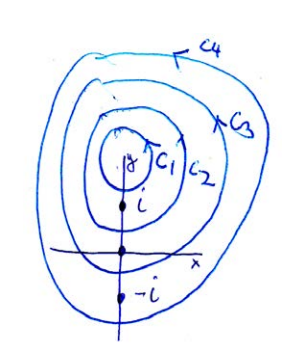
\includegraphics[width=0.5\linewidth]{Screenshot 2025-09-11 012149.png}
    \end{figure}
\end{frame}
\begin{frame}{Example}
    Evaluate $$\oint_C \frac{2+3\sin(\pi z)}{z(z-1)^2}dz$$
    where $C$ is a square having vertices at $3+3i$, $3-3i$, $-3+3i$ and $-3-3i$.
\end{frame}

\end{document}